\subsection{Case 0, $M=N$}
The results are plotted for data set S1\_Cclean. The data set consist of 144 time segment with $L_s = 516$ samples and $M\_ = 27$ sensors. Figure \ref{fig:M=N_1} show $MSE\left(\hat{\mathbf{X}}_{\text{main}},\hat{\mathbf{X}}_{\text{ICA}}\right)$ for all segments $s$. ICA is applied on $\textbf{Y}_s$ specified by $M\_ = 27$ and $L_s = 516$. The main algorithm is applied on $\textbf{Y}_s$ without any reduction hence specified by $M=27$ and $L_s=516$, given $\textbf{A}_{fix}$ and $N = k$ provided from ICA.
Figure \ref{fig:M=N_1_2} show the same plot but the y-axis is specified to the interval [-10,50] for better visualization.
Furthermore is the MSE tolerance $= 5$ plotted, indicting for each segment whether the estimate $\hat{\mathbf{X}}_{\text{main}}$ is sufficiency close to $\hat{\mathbf{X}}_{\text{main}}$. It is seen that for a majority of the segments the MSE lies under the tolerance, but single outliers appears for which the MSE of the segment is remarkably increased.    
\begin{figure}[H]
\begin{widepage}
    \begin{minipage}[t]{.45\textwidth}
		\centering
		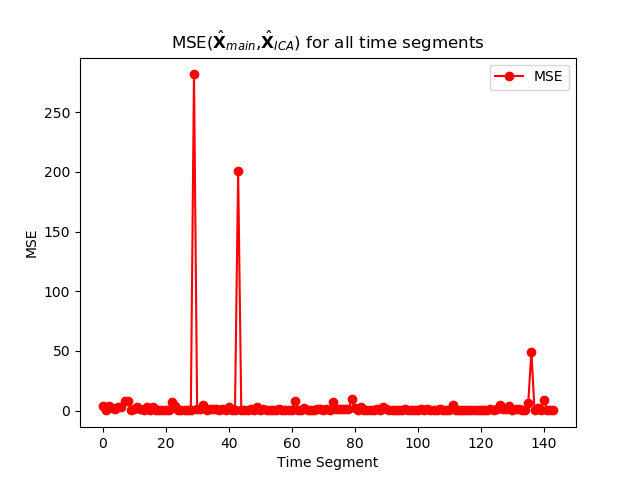
\includegraphics[width=1\linewidth]{figures/ch_7/resultat/average_mse_none_removed_ica}
	\caption{$MSE\left(\hat{\mathbf{X}}_{\text{main}},\hat{\mathbf{X}}_{\text{ICA}}\right)$ for all 144 segments}
	\label{fig:M=N_1}
    \end{minipage} 
    \hspace{0.5cm}
    \begin{minipage}[t]{.45\textwidth}
        \centering
		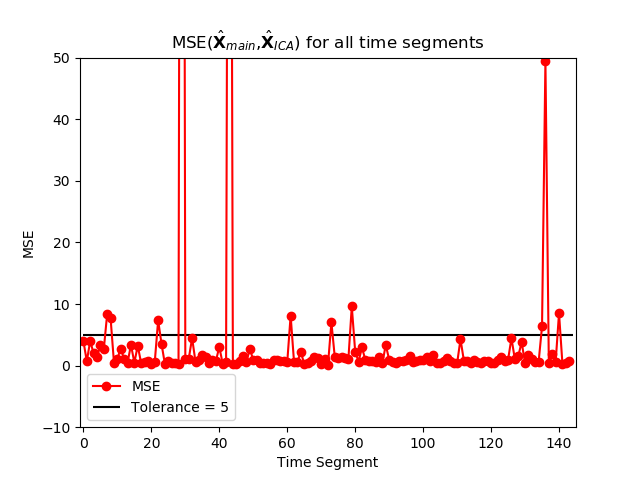
\includegraphics[width=1\linewidth]{figures/ch_7/resultat/average_mse_none_removed_ica_zoom.png}
	\caption{$MSE\left(\hat{\mathbf{X}}_{\text{main}},\hat{\mathbf{X}}_{\text{ICA}}\right)$ for all 144 segments. Plotted only for the y-axis interval [-10, 50] for better visualisation.}
	\label{fig:M=N_1_2}
    \end{minipage}
\end{widepage}
\end{figure}
To investigate the behaviour of a single segment figure \ref{fig:M=N_2} show the MSE value computed for each row of the two estimates of a specific segment. That is $MSE\left(\hat{\mathbf{X}}_{\text{main}_{i}},\hat{\mathbf{X}}_{\text{ICA}_{i}}\right)$ for every row $i = 1, \hdots, k$ in time segment $s=56$. Additionally figure \ref{fig_M=N} show and compare the corresponding estimates for four random chosen sources. This allows for visual comparison of the estimates relative to the corresponding MSE value seen in figure \ref{fig:M=N_2}. Note that for better visual comparison each plotted row of $\hat{\textbf{X}}_{ICA}$ is scaled with respect to the max value of the corresponding row in $\hat{\textbf{X}}_{Main}$.
From figure \ref{fig:M=N_2} it is seen that the estimate of each source result in a relative low MSE which indicate that the main algorithm has managed to estimate the same source as the ICA algorithm. In contradiction to this, figure \ref{fig:M=N_3} do not confirm that the estimates are close, as generally the two signals in one plot does not follow the same trend.   
\begin{figure}[H]
\begin{widepage}
    \begin{minipage}[t]{.45\textwidth}
\centering
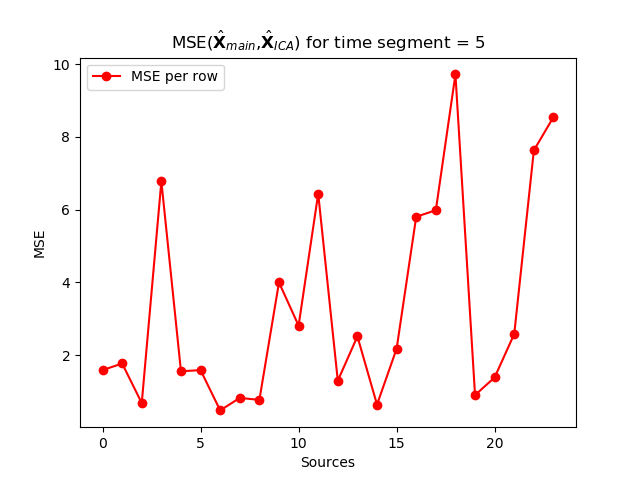
\includegraphics[width=1\linewidth]{figures/ch_7/resultat/mse_none_removed_ica_timeseg5.png}
\caption{$MSE\left(\hat{\mathbf{X}}_{\text{main}_{i}},\hat{\mathbf{X}}_{\text{ICA}_{i}}\right)$ for every row $i = 1, \hdots, k$ in time segment $s=56$.}
\label{fig:M=N_2}
\end{minipage} 
\hspace{0.5cm}
\begin{minipage}[t]{.45\textwidth}
\centering
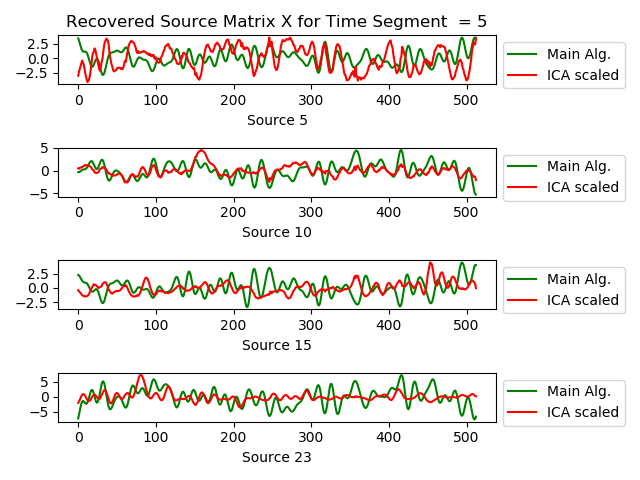
\includegraphics[width=1\linewidth]{figures/ch_7/resultat/EEG_none_removed_scaled_timeseg5S1_CClean.png}
\caption{Plot of the $k = 13$ sources from $\hat{\mathbf{X}}_{\text{main}}$ and $\hat{\mathbf{X}}_{\text{ICA}}$ from time segment $s = 56$ with $M=N$}
	\label{fig:M=N_3}
    \end{minipage}
\end{widepage}
\end{figure}
The test is repeated for every data set, and the results are summarised in table \ref{tab:case_0}. In general a low MSE is achieved in average over all segments of one data set, relative to the tolerance, and the corresponding percentage is likewise relative high, with an average at $83\%$. A single result is seen to deviate from the tendency, the data set of test subject 3 with closed eyes. Here a remarkably high average MSE value is found, indicating that a majority of the segment has resulted in a significantly high MSE, while a percentage of $???$ was below the tolerance.  
In chapter \ref{ch:implementation} it is found that the the main algorithm was capable of providing an almost exact estimate for $M=N$ when the true $\textbf{A}$ is provided. Thus it is expected that the general performance is decreased in this case where the true $\textbf{A}$ in unknown and $\textbf{A}_{fix}$ is given.
The achieved results will serve as reference when analysing the results of the following cases where the main algorithm is applied on data set reduced with respect to the original data set.       
\begin{table}[]
\centering
\begin{tabular}{|c|c|c|c|c|c|c|}
\hline
\multirow{2}{*}{\textbf{\begin{tabular}[c]{@{}c@{}}Case 0 \\ $M=N$\end{tabular}}} & \multicolumn{2}{c|}{test subject 1} & \multicolumn{2}{c|}{test subject 2} & \multicolumn{2}{c|}{test subject 3} \\ \cline{2-7} 
                                                                                  & Open             & Close            & Open             & Close            & Open            & Close             \\ \hline
\multicolumn{1}{|c|}{Average MSE()}                                               & 2.913            & 5.172            & 1.572            & 15.06            & 4.753            & 19.44           \\ \hline
\begin{tabular}[c]{@{}c@{}}Segments below \\ tolerance in \%\end{tabular}          & 91             & 92            & 98 & 61             & 87            & 63 \\ \hline
\end{tabular}
\caption{Summarised results for Case 0. Test is performed on the every data set.}
\label{tab:case_0}
\end{table}	


\subsection{Case 1, $M<N$}
Here the main algorithm is applied to a data set, where the number of sensors is reduced by one third. As such ICA is applied on the original data set with segments $\textbf{Y}_s$ specified by $M_= 27$ and $L_s = 516$. The main algorithm is applied on $\textbf{Y}_s$ specified by $M=18$ and $L_s=516$, given $\textbf{A}_{fix}$ and $N = k$ provided from ICA.  
The viewed plots correspond to those of case 0, but for reduce number of sources $M<N$, hence detailed plot description is omitted here.   

From figure \ref{fig:M<N_1} and \ref{fig:M<N_1_2} it is seen that the for a majority of the segments the MSE value is close to the tolerance, but the number of outliers has increased compared to case 0, indicating the that for an increased number of segments the main algorithm do not manage to estimate enough  sources sufficiently in order to stay below the tolerance.   
\begin{figure}[H]
\begin{widepage}
    \begin{minipage}[t]{.45\textwidth}
		\centering
		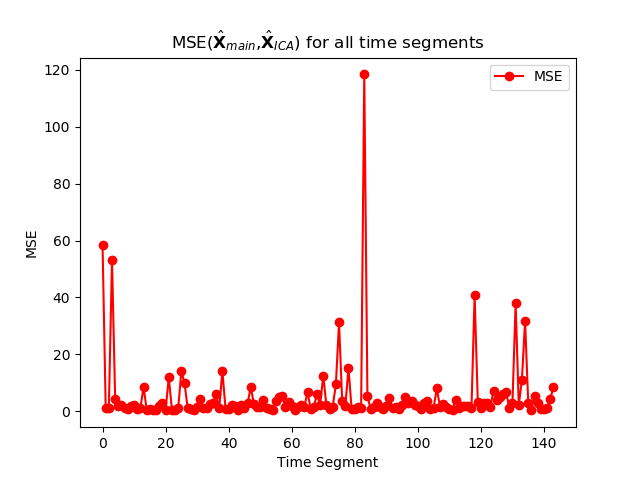
\includegraphics[width=1\linewidth]{figures/ch_7/resultat/average_mse_third_removed_ica}
	\caption{$MSE\left(\hat{\mathbf{X}}_{\text{main}},\hat{\mathbf{X}}_{\text{ICA}}\right)$ for all 144 segments}
	\label{fig:M<N_1}
    \end{minipage} 
\hspace{0.5cm}
    \begin{minipage}[t]{.45\textwidth}
        \centering
		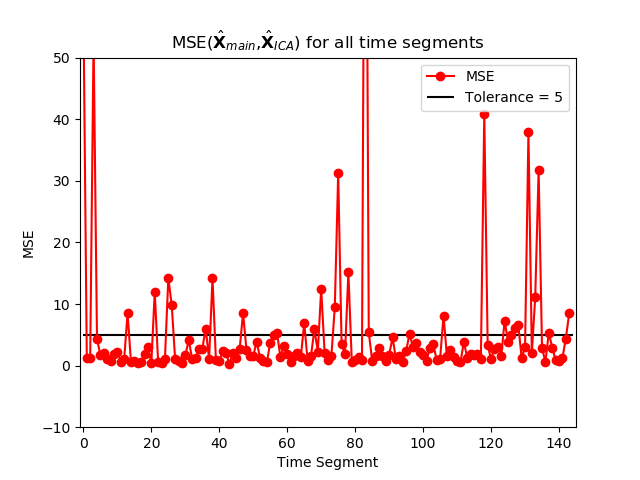
\includegraphics[width=1\linewidth]{figures/ch_7/resultat/average_mse_third_removed_ica_zoom.png}
	\caption{$MSE\left(\hat{\mathbf{X}}_{\text{main}},\hat{\mathbf{X}}_{\text{ICA}}\right)$ for all 144 segments. Plotted only for the y-axis interval [-10, 50] for better visualisation.}
	\label{fig:M<N_1_2}
    \end{minipage}
\end{widepage}
\end{figure}
\noindent 
From figure \ref{fig:M<N_2} and \ref{fig:M<N_3} showing the results of segment 56, it is seen that the MSE for each source has increased slightly compare to case 0. This supports the observation from figure \ref{fig:M<N_1_2}.      
\begin{figure}[H]
\begin{widepage}
    \begin{minipage}[t]{.45\textwidth}
\centering
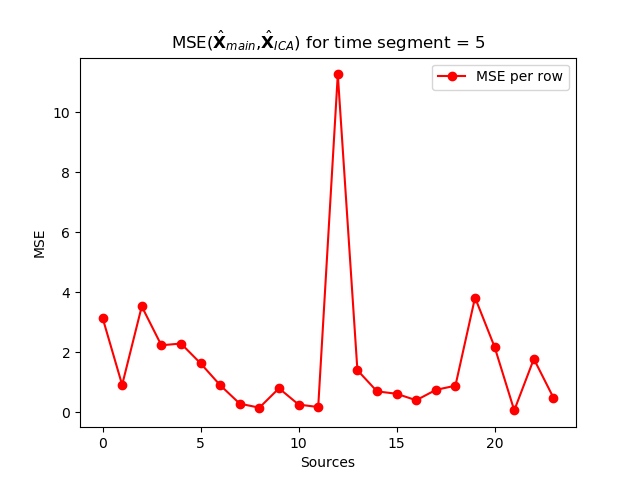
\includegraphics[width=1\linewidth]{figures/ch_7/resultat/mse_third_removed_ica_timeseg5.png}
\caption{$MSE\left(\hat{\mathbf{X}}_{\text{main}_{i}},\hat{\mathbf{X}}_{\text{ICA}_{i}}\right)$ for every row $i = 1, \hdots, k$ in time segment $s=56$.}
\label{fig:M<N_2}
\end{minipage} 
\hspace{0.5cm}
\begin{minipage}[t]{.45\textwidth}
\centering
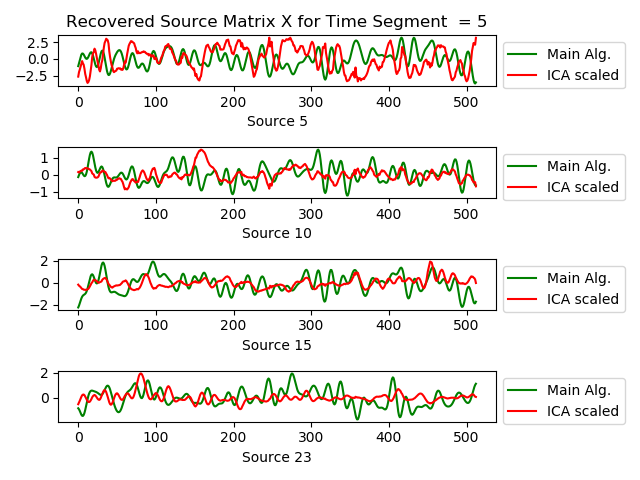
\includegraphics[width=1\linewidth]{figures/ch_7/resultat/EEG_third_removed_scaled_timeseg5S1_CClean.png}
\caption{Plot of the $k = 13$ sources from $\hat{\mathbf{X}}_{\text{main}}$ and $\hat{\mathbf{X}}_{\text{ICA}}$ from time segment $s = 56$ with $M=N$}
	\label{fig:M<N_3}
    \end{minipage}
\end{widepage}
\end{figure}
The test is repeated for every data set, and the results are summarised in table \ref{tab:case_1}. Comparing table \ref{tab:case_1} to table \ref{tab:case_0}, summarising the results of case 0, it is seen that the percentage of segments below the tolerance are decreasing, with the majority being close to 50\%, thoroughly indicating that half of the time the main algorithm do not manage to provide a sufficient estimate when $M = 2/3N$.  
Furthermore both the average MSE and the corresponding percentage appears fluctuating relative to case 0 indicating some unreliability in the results.  

\begin{table}[h]
\centering
\begin{tabular}{|c|c|c|c|c|c|c|}
\hline
\multirow{2}{*}{\textbf{\begin{tabular}[c]{@{}c@{}}Case 1 \\ $M<N$\end{tabular}}} & \multicolumn{2}{c|}{test subject 1} & \multicolumn{2}{c|}{test subject 2} & \multicolumn{2}{c|}{test subject 3} \\ \cline{2-7} 
                                                                                  & Open             & Close            & Open             & Close            & Open              & Close           \\ \hline
\multicolumn{1}{|c|}{Average MSE()}                                               & 9.79            & 5.351            & 13.89            & 15.13            & 6.25          & 18.21          \\ \hline
\begin{tabular}[c]{@{}c@{}}Segments below \\ tol in percent\end{tabular}          & 53             & 80             & 66 & 46             & 77              & 48            \\ \hline
\end{tabular}
\caption{Summarised results for Case 1. Test is performed on the every data set.}
\label{tab:case_1}
\end{table}

\subsection{Case 2, $M<<N$}
Here the main algorithm is applied to a data set, where the number of sensors is reduced to half. As such ICA is applied on the original data set with segments $\textbf{Y}_s$ specified by $M_= 27$ and $L_s = 516$. The main algorithm is applied on $\textbf{Y}_s$ specified by $M=13$ and $L_s=516$, given $\textbf{A}_{fix}$ and $N = k$ provided from ICA.  
The viewed plots correspond to those of case 0 and case 1, but for further reduce number of sources $M<<N$, hence detailed plot description is omitted.   

From figure \ref{fig:M<<N_1} and \ref{fig:M<<N_1_2} it is seen that the MSE value for each segment is more widely scatted around the tolerance, compared to case 0 and 1. Outliers where the MSE value has increased significantly do also occur, similar to case 1. This indicates that the performance of the main algorithm has decreased further, compared to case 1. 

\begin{figure}[H]
\begin{widepage}
    \begin{minipage}[t]{.45\textwidth}
		\centering
		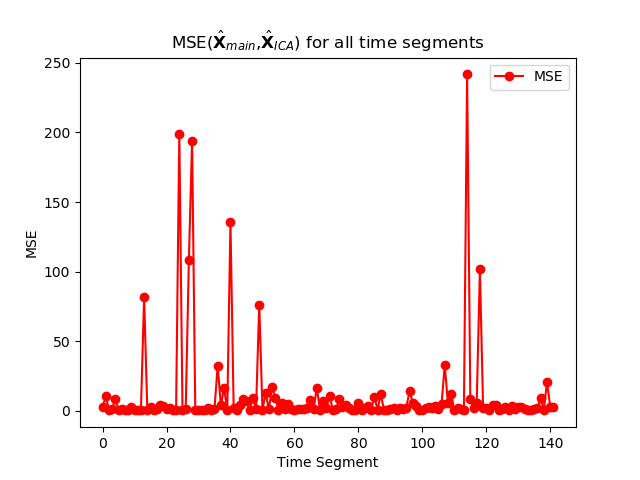
\includegraphics[width=1\linewidth]{figures/ch_7/resultat/average_mse_second_removed_ica}
	\caption{$MSE\left(\hat{\mathbf{X}}_{\text{main}},\hat{\mathbf{X}}_{\text{ICA}}\right)$ for all 144 segments}
	\label{fig:M<<N_1}
    \end{minipage} 
\hspace{0.5cm}
    \begin{minipage}[t]{.45\textwidth}
        \centering
		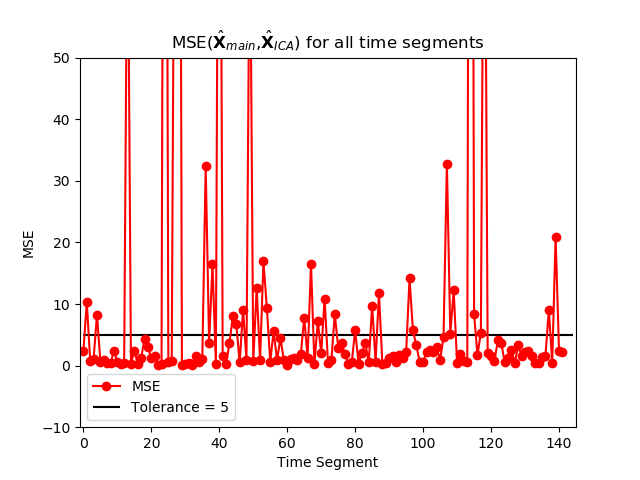
\includegraphics[width=1\linewidth]{figures/ch_7/resultat/average_mse_second_removed_ica_zoom.png}
	\caption{$MSE\left(\hat{\mathbf{X}}_{\text{main}},\hat{\mathbf{X}}_{\text{ICA}}\right)$ for all 144 segments. Plotted only for the y-axis interval [-10, 50] for better visualisation.}
	\label{fig:M<<N_1_2}
    \end{minipage}
\end{widepage}
\end{figure}
\noindent 
The above indication is supported by figure \ref{fig:M<<N_2} and \ref{fig:M<<N_3} showing an general increase in MSE. However segment 56 still makes a fairly good example as the majority of the sources have achieves a MSE below the tolerance of 5. From figure \ref{fig:M<<N_3} the increased MSE do not appear visually compare to either case 1 or case 0.        
\todo{tjek source nr. i label på alle signal plottene det stemmer ikke her }
\begin{figure}[H]
\begin{widepage}
    \begin{minipage}[t]{.49\textwidth}
\centering
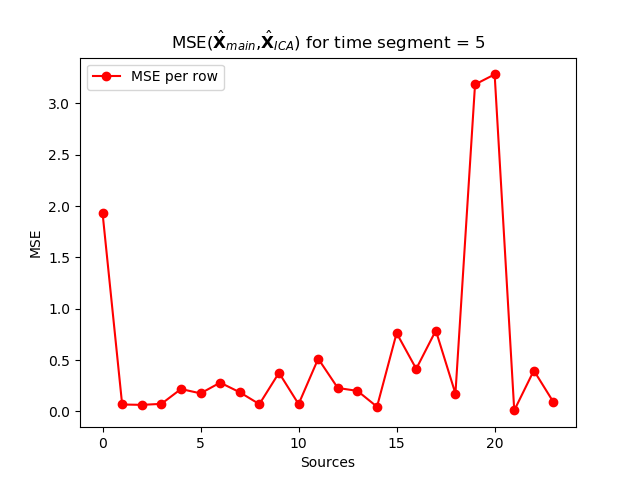
\includegraphics[width=1\linewidth]{figures/ch_7/resultat/mse_second_removed_ica_timeseg5.png}
\caption{$MSE\left(\hat{\mathbf{X}}_{\text{main}_{i}},\hat{\mathbf{X}}_{\text{ICA}_{i}}\right)$ for every row $i = 1, \hdots, k$ in time segment $s=56$.}
\label{fig:M<<N_2}
\end{minipage} 
\hspace{.5cm}
\begin{minipage}[t]{.49\textwidth}
\centering
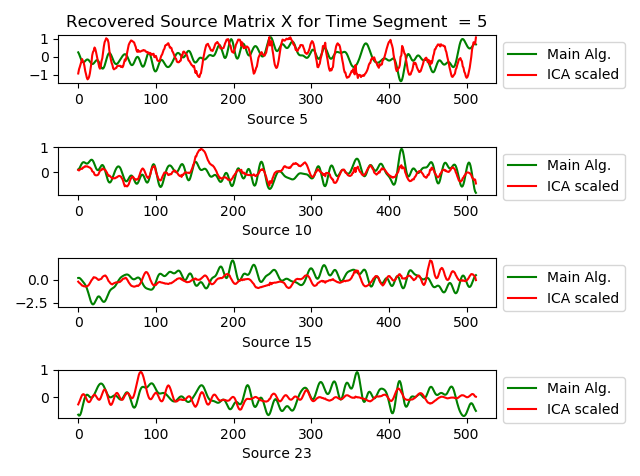
\includegraphics[width=1\linewidth]{figures/ch_7/resultat/EEG_second_removed_scaled_timeseg5S1_CClean.png}
\caption{Plot of the $k = 13$ sources from $\hat{\mathbf{X}}_{\text{main}}$ and $\hat{\mathbf{X}}_{\text{ICA}}$ from time segment $s = 56$ with $M<N$}
	\label{fig:M<<N_3}
    \end{minipage}
\end{widepage}
\end{figure}

The test is repeated for every data set, and the results are summarised in table \ref{tab:case_2}. Comparing table \ref{tab:case_0} to table \ref{tab:case_1}, summarising the results of case 1, it is generally seen that the percentage of segments below the tolerance is not decreased but improved, though without getting close to the tendency from case 0. Furthermore the average MSE has not increased remarkably compared to case 1. As such the performance of the main algorithm in case 2 is in general not found to be worse than for case 1, however a clear improvement is not seen either.  



\begin{table}[]
\centering
\begin{tabular}{|c|c|c|c|c|c|c|}
\hline
\multirow{2}{*}{\textbf{\begin{tabular}[c]{@{}c@{}}Case 2\\ $M<<N$\end{tabular}}} & \multicolumn{2}{c|}{test subject 1} & \multicolumn{2}{c|}{test subject 2} & \multicolumn{2}{c|}{test subject 3} \\ \cline{2-7} 
                                                                                  & Open             & Close            & Open             & Close            & Open             & Close            \\ \hline
\multicolumn{1}{|c|}{Average MSE()}                                               & 8.378            & 11.36            & 19.58            & 13.11            & 13.99           & 11.96            \\ \hline
\begin{tabular}[c]{@{}c@{}}Segments below \\ tol in percent\end{tabular}          & 75             & 74             & 42 & 72             & 69             & 69 \\ \hline
\end{tabular}
\caption{Summarised results for case 2. Test is performed on the every data set.}
\label{tab:case_2}
\end{table}
